\documentclass[tikz, border=10pt]{standalone}
\usepackage{amsmath,amssymb}
\usetikzlibrary{arrows.meta}

\begin{document}

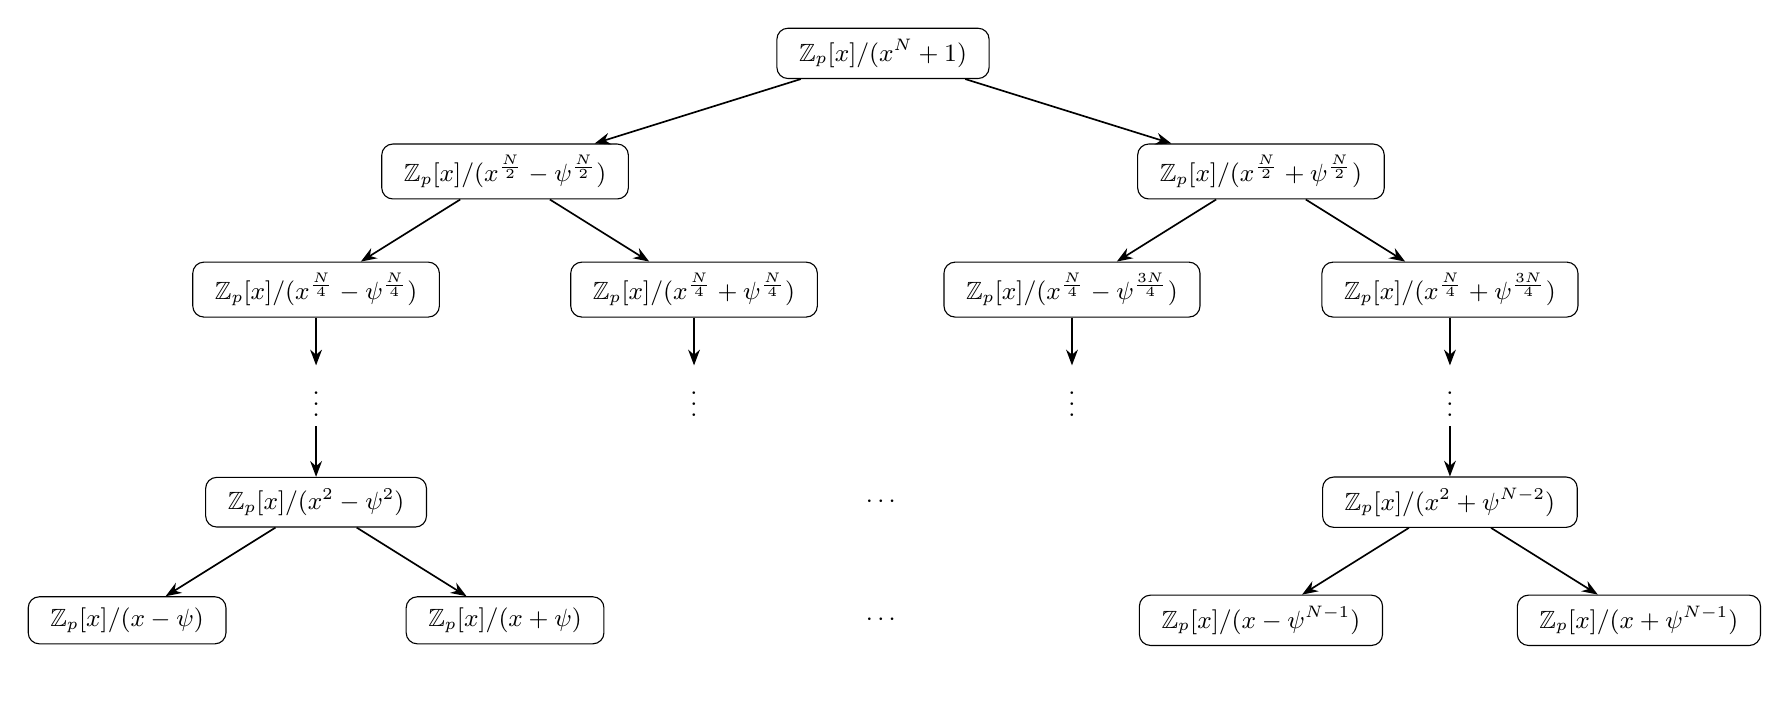
\begin{tikzpicture}[>=Stealth, font=\small]

\tikzset{
  box/.style={draw, rounded corners, align=center, inner xsep=8pt, inner ysep=4pt},
  arr/.style={->, line width=0.6pt}
}

% --- Nós (Coordenadas fixas para layout simétrico) ---
% Raiz: Polinômio Negacíclico original
\node[box] (root) at (0,0) {$\mathbb{Z}_p[x]/(x^{N}+1)$};

% Nível 1: Decomposição em N/2
% Lembra que x^N + 1 = x^N - \psi^N = (x^{N/2} - \psi^{N/2})(x^{N/2} + \psi^{N/2})
\node[box] (L1) at (-4.8,-1.5) {$\mathbb{Z}_p[x]/(x^{\frac N2}-\psi^{\frac N2})$};
\node[box] (R1) at ( 4.8,-1.5) {$\mathbb{Z}_p[x]/(x^{\frac N2}+\psi^{\frac N2})$};

% Nível 2: Decomposição em N/4
\node[box] (L2a) at (-7.2,-3.0) {$\mathbb{Z}_p[x]/(x^{\frac N4}-\psi^{\frac N4})$};
\node[box] (L2b) at (-2.4,-3.0) {$\mathbb{Z}_p[x]/(x^{\frac N4}+\psi^{\frac N4})$};

\node[box] (R2a) at ( 2.4,-3.0) {$\mathbb{Z}_p[x]/(x^{\frac N4}-\psi^{\frac{3N}{4}})$};
\node[box] (R2b) at ( 7.2,-3.0) {$\mathbb{Z}_p[x]/(x^{\frac N4}+\psi^{\frac{3N}{4}})$};

% Elipses Verticais (indicando recursão)
\node (vdL2a) at (-7.2,-4.35) {$\vdots$};
\node (vdL2b) at (-2.4,-4.35) {$\vdots$};
\node (vdR2a) at ( 2.4,-4.35) {$\vdots$};
\node (vdR2b) at ( 7.2,-4.35) {$\vdots$};

% Exemplos da Base (apenas as pontas esquerda e direita para simplificar)
% Nível N-2
\node[box] (BLmid) at (-7.2,-5.7) {$\mathbb{Z}_p[x]/(x^{2}-\psi^{2})$};
\node[box] (BRmid) at ( 7.2,-5.7) {$\mathbb{Z}_p[x]/(x^{2}+\psi^{N-2})$};

% Nível Final (Grau 1 - Fatores Lineares)
% Esquerda: Raiz \psi^1
\node[box] (BL1) at (-9.6,-7.2) {$\mathbb{Z}_p[x]/(x-\psi)$};
\node[box] (BL2) at (-4.8,-7.2) {$\mathbb{Z}_p[x]/(x+\psi)$};

% Direita: Raiz \psi^{N-1} (Note que x + \psi^{N-1} corresponde a raiz -\psi^{N-1})
\node[box] (BR1) at ( 4.8,-7.2) {$\mathbb{Z}_p[x]/(x-\psi^{N-1})$};
\node[box] (BR2) at ( 9.6,-7.2) {$\mathbb{Z}_p[x]/(x+\psi^{N-1})$};

% Elipses Horizontais
\node at (0,-5.7) {$\cdots$};
\node at (0,-7.2) {$\cdots$};

% --- Setas ---
\draw[arr] (root) -- (L1);
\draw[arr] (root) -- (R1);

\draw[arr] (L1) -- (L2a);
\draw[arr] (L1) -- (L2b);

\draw[arr] (R1) -- (R2a);
\draw[arr] (R1) -- (R2b);

\draw[arr] (L2a) -- (vdL2a);
\draw[arr] (L2b) -- (vdL2b);
\draw[arr] (R2a) -- (vdR2a);
\draw[arr] (R2b) -- (vdR2b);

% Conexões das pontas
\draw[arr] (vdL2a) -- (BLmid);
\draw[arr] (BLmid) -- (BL1);
\draw[arr] (BLmid) -- (BL2);

\draw[arr] (vdR2b) -- (BRmid);
\draw[arr] (BRmid) -- (BR1);
\draw[arr] (BRmid) -- (BR2);

% --- Legenda Falsa (Node) ---
\node[below=0.5cm] at (0,-7.2) {};

\end{tikzpicture}

\end{document}